\documentclass[border=12pt]{standalone}
\usepackage[utf8]{inputenc}
\usepackage[utf8]{vietnam} %Bien dich duoc tieng Viet
\usepackage{amsmath,amsfonts,amssymb} %Font toan
\usepackage{tikz}
\usetikzlibrary{arrows, decorations.markings, calc, fadings, decorations.pathreplacing, patterns, decorations.pathmorphing, positioning}
%\tikzstyle{every path}=[line width=1.2pt]
\newcommand{\drawe}{\draw[line width=1.2pt]}
\newcommand{\bigf}[1]{\Large{#1}} % Ký hiệu cho máy phát
\newcommand{\bbigf}[1]{\huge{#1}} % Tên của các phần tử
\begin{document}
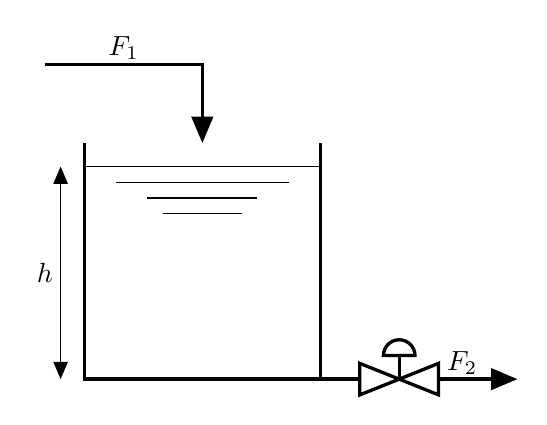
\begin{tikzpicture}[>=triangle 45]
%\draw[color=blue] (-2,-2) grid (11,11); %Tạo lưới
% Vẽ bình chứa
\drawe (0,3) -- (0,0) -- (3,0) -- (3,3);
\draw (0,2.7) -- (3,2.7);
\draw (0.4,2.5) -- (2.6, 2.5);
\draw (0.8,2.3) -- (2.2, 2.3);
\draw (1,2.1) -- (2, 2.1);
\drawe (-.5, 4) -- (1.52,4);
\drawe[->] (1.5, 4) -- (1.5, 3);

\draw (0.5,4.2) node{$F_1$};

\draw[<->] (-0.3,0) -- (-0.3,2.7);
\draw (-0.5, 1.35) node {$h$};


% Vẽ van điều khiển ngõ ra
\drawe (3,0) -- (3.5,0);
\drawe (3.5,0) -- (3.5,-.2) -- (4.5,0.2) -- (4.5,-.2) -- (3.5,.2) -- (3.5,0);
\drawe (4,0) -- (4, .3);
\drawe (4.2,.3) arc (0:180:.2) -- (4.22,.3);
\drawe[->] (4.5,0) -- (5.5,0);
\draw (4.8,.2) node{$F_2$};

\end{tikzpicture}
\end{document}